\subsection{Correctness and certificate tightness}\label{sec:accuracy}
All 38 formula checks and the 46 tests of Appendix~\ref{app:verification} pass. At scale, we compared the walk sum on the thermal grid ($N=9.1\times10^4$) and on the random network ($N=2^{16}$, degrees 4 and 16) with \texttt{expm\_multiply} applied to the exported matrix, for pruning thresholds $\tau=10^{-4},\dots,10^{-12}$. Of the 35 runs, 33 finished and two (the grid at $\mu=0.76$ and the degree-16 network at $\mu=0.57$, both at $\tau=10^{-12}$) reached the 300~s time limit, in which case no certificate is issued. In all 33 finished runs the observed maximum error over the time grid lay below the certificate (Fig.~\ref{fig:certificate}). The certificates are conservative, and how conservative depends strongly on the graph. On the grid the ratio of certificate to observed error was 5 to 34 for the step response and 28 to 344 for the impulse kernel. On the random networks it was 8 to $1.1\times10^4$ for the step response and 39 to $7.6\times10^4$ for the kernel, growing with the degree and with $\mu$. The reason is visible in the bound itself: it charges every discarded walk as if it could still return to the sensor, with the comparison ratio as the only attenuation per step. On a lattice a discarded walk has a fair chance of returning; on a locally tree-like graph of degree $\Delta$ the chance of stepping back toward the sensor is about $1/\Delta$ per step, which the bound ignores. For the real, nonnegatively coupled models of this section all walk contributions have the same sign, so the cancellation indicator is exactly one.

The certificate does not cover rounding, so we tested the temporal kernel separately on directed chains $\dot x_i=d_ix_i+x_{i-1}$, whose single walk from the first to the last state makes the output equal to one divided difference, compared with 60-digit evaluations at 50 sampled times. Five node sets were used: two and four distinct real nodes, a stiff set spread over four decades ($-0.5$ to $-5000$), seven clustered and repeated nodes (spacing $10^{-9}$), and complex nodes. With a fixed horizon $t\le10$ and $T=10^2$ to $10^5$ samples, the largest relative errors of the kernel grew from about $10^{-15}$ to $3\times10^{-12}$; with a fixed step $\Delta t=0.05$ and horizons up to 500, the stiff set reached $3.8\times10^{-11}$ at $T=10^4$. This is the roughly linear growth with the number of steps expected from Sec.~\ref{sec:kernel}, at a level far below the truncation certificates used here (data in \texttt{kernel\_long\_grid.json}).

\begin{figure}[t]
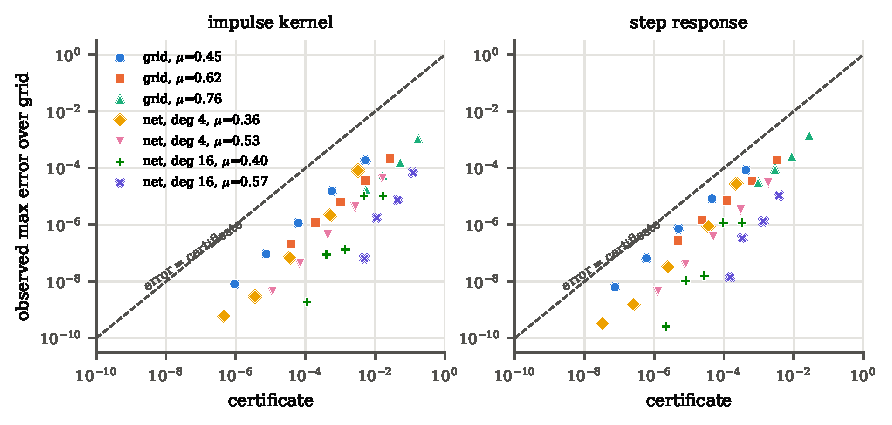
\includegraphics[width=\linewidth]{figures/fig_certificate.pdf}
\caption{Observed maximum error over the time grid against the a posteriori certificate, for the impulse kernel (left) and the step response (right), over pruning thresholds $\tau=10^{-4}$ to $10^{-12}$. Points below the dashed line are certified. Grid: $301\times301$ thermal network; net: random network with $2^{16}$ states. Reference: \texttt{expm\_multiply} on the full matrix.}\label{fig:certificate}
\end{figure}

\subsection{Memory and time versus state dimension}\label{sec:scaling}
Table~\ref{tab:scaling} and Fig.~\ref{fig:scaling} fix the query (collocated sensor and actuator, impulse kernel and step response, $\tau=10^{-10}$) and vary $N$: the thermal grid from $10^4$ to $10^{12}$ states and the degree-4 random network from $2^{16}$ to $2^{64}$. The thermal parameters are hashed from coordinates centered on the sensor, so the neighborhood of the sensor is the same at every size, and the random network is locally tree-like at every size, so the work of the walk sum should not depend on $N$. It does not. On the grid the traversal took 0.07~s and visited $1.10$ to $1.15\times10^5$ walk prefixes at every size (the small variation comes from the global bounds, which are maxima over all states), and on the network 0.02~s with $6.0$ to $7.2\times10^4$ prefixes; the peak memory of the process was 4.5 to 4.6~MB throughout. The global constants needed by the certificate were computed by a streaming pass over all states for the grid up to $10^7$ states, which took 1.1~s at $N=10^7$ and is not included in the traversal time, and from the parameter ranges otherwise.

The global methods behave as expected of state-vector methods. \texttt{expm\_multiply} on the full matrix took 0.5, 5.3, 50 and 634~s on the grid from $10^4$ to $10^7$ states and 4.6, 27, 161 and 911~s on the network from $2^{16}$ to $2^{22}$; the Arnoldi method was slower still. At $N=10^7$ its peak was 2.9~GB above the import baseline. Of this, the matrix itself accounts for 0.6~GB and most of the rest is a shifted copy of the matrix that SciPy forms internally, so a leaner implementation would need about 1~GB (the matrix and a few state vectors), still more than two orders of magnitude above the walk sum. Larger sizes were not run: at $N\ge2^{32}$ and $N\ge10^{10}$ the state vector alone exceeds the memory of the machine, and the network at $2^{24}$ was skipped for run time. All global results agreed with the walk sum to within 0.19 of its certificate. The certified ball at the walk sum's certificate has 113 states on the grid and about 1460 on the network, independent of $N$; solved by \texttt{expm\_multiply} it took 0.2 to 0.3~s and about 1~MB above the import baseline, most of the time being interpreter overhead. At these small coupling ratios both the walk sum and the ball are cheap, and the comparison that matters is the one of the next section.

\begin{table*}[t]
\footnotesize\setlength{\tabcolsep}{4pt}
\caption{Time [s] and memory [MB] versus state dimension at fixed query and pruning threshold ($\tau=10^{-10}$). Walk sum: peak memory of the C++ process. Python methods: peak minus the high-water mark after importing NumPy and SciPy (about 57~MB). Ball: certified ball at the walk sum's certificate, solved by \texttt{expm\_multiply}. n.r.: not run (state-vector methods beyond the tested range, or Krylov beyond $10^6$).}\label{tab:scaling}
\begin{ruledtabular}
\begin{tabular}{ll|cc|cc|cc|cc}
model & $N$ & \multicolumn{2}{c|}{walk sum} & \multicolumn{2}{c|}{ball + expm\_multiply} & \multicolumn{2}{c|}{expm\_multiply (full)} & \multicolumn{2}{c}{Arnoldi $m=30$ (full)}\\
 & & time [s] & mem. [MB] & time [s] & mem. [MB] & time [s] & mem. [MB] & time [s] & mem. [MB]\\\hline
thermal grid & 1.0e4 & 0.07 & 4.5 & 0.22 & 0.9 & 0.51 & 4.9 & 1.20 & 5.4 \\
thermal grid & 1.0e5 & 0.07 & 4.5 & 0.19 & 1.0 & 5.28 & 33.0 & 19 & 35.6 \\
thermal grid & 1.0e6 & 0.07 & 4.5 & 0.18 & 1.0 & 50 & 311.0 & 227 & 342.3 \\
thermal grid & 1.0e7 & 0.07 & 4.5 & 0.23 & 0.9 & 634 & 2943.6 & n.r. & n.r. \\
thermal grid & 1.0e10 & 0.07 & 4.5 & 0.26 & 1.0 & n.r. & n.r. & n.r. & n.r. \\
thermal grid & 1.0e12 & 0.07 & 4.5 & 0.31 & 0.9 & n.r. & n.r. & n.r. & n.r. \\
random net, $\Delta=4$ & $2^{16}$ & 0.02 & 4.5 & 0.30 & 1.2 & 4.59 & 21.6 & 8.65 & 23.6 \\
random net, $\Delta=4$ & $2^{18}$ & 0.02 & 4.5 & 0.28 & 1.2 & 27 & 82.6 & 39 & 88.9 \\
random net, $\Delta=4$ & $2^{20}$ & 0.03 & 4.5 & 0.29 & 1.2 & 161 & 325.5 & 243 & 357.9 \\
random net, $\Delta=4$ & $2^{22}$ & 0.02 & 4.5 & 0.29 & 1.2 & 911 & 1281.6 & n.r. & n.r. \\
random net, $\Delta=4$ & $2^{24}$ & 0.02 & 4.5 & 0.32 & 1.2 & n.r. & n.r. & n.r. & n.r. \\
random net, $\Delta=4$ & $2^{32}$ & 0.02 & 4.5 & 0.31 & 1.2 & n.r. & n.r. & n.r. & n.r. \\
random net, $\Delta=4$ & $2^{48}$ & 0.02 & 4.5 & 0.30 & 1.2 & n.r. & n.r. & n.r. & n.r. \\
random net, $\Delta=4$ & $2^{64}$ & 0.02 & 4.5 & 0.28 & 1.2 & n.r. & n.r. & n.r. & n.r. \\
\end{tabular}
\end{ruledtabular}
\end{table*}


\begin{figure}[t]
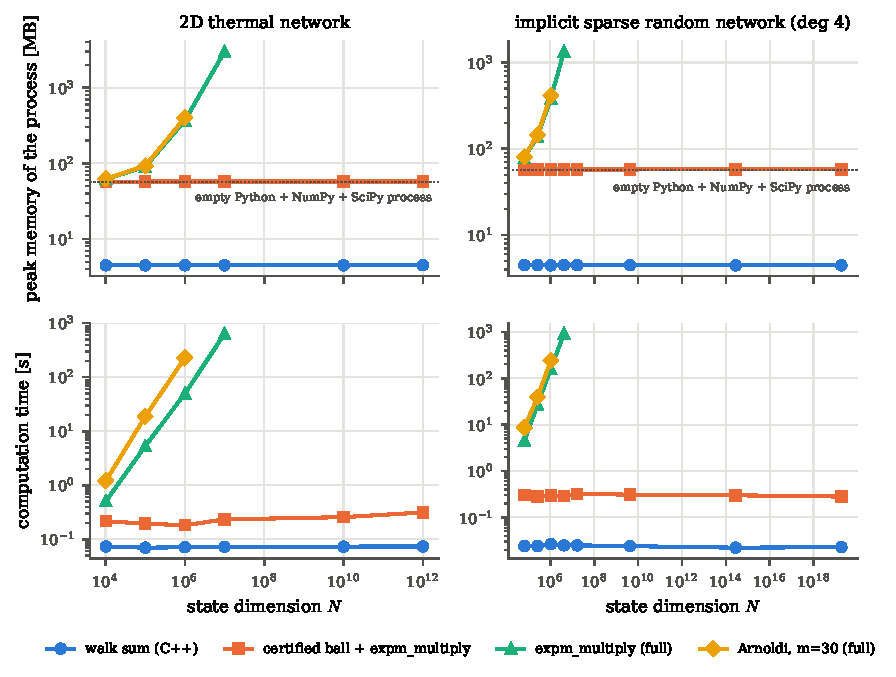
\includegraphics[width=\linewidth]{figures/fig_scaling.pdf}
\caption{Peak memory of the whole process (top) and computation time (bottom) against the state dimension, for the thermal grid ($\mu=0.45$) and the degree-4 random network ($\mu=0.36$) at fixed pruning threshold $\tau=10^{-10}$. Full-system methods were run up to $10^7$ (grid) and $2^{22}$ (network) states; larger sizes were not run. The dotted line marks the peak of a Python process that has imported NumPy and SciPy and holds no data. Data in Table~\ref{tab:scaling}.}\label{fig:scaling}
\end{figure}

\subsection{Walk sums versus certified local truncations}\label{sec:crossover}
Global methods are not the strongest competitors. A local method that propagates the state only on a set of states around the actuator has memory proportional to that set, and with the certificates of Sec.~\ref{sec:local} it carries the same guarantee as the walk sum. Table~\ref{tab:crossover} and Fig.~\ref{fig:crossover} compare the walk sum with the certified ball and the adaptive set at matched targets $10^{-3}$, $10^{-4}$ and $10^{-5}$ for the step response. The comparison covers the random network with $N=2^{64}$ at degrees 4, 16 and 32 with two values of $\mu$ each, and the thermal grid with two values of $\mu$. All three methods use the same distance information and the same compiler, and run single-threaded; the walk sum is charged the full time of its threshold search. In every case where two methods both reached the target, their outputs agreed within the sum of their certificates.

\begin{table*}[t]
\footnotesize\setlength{\tabcolsep}{1.35pt}
\caption{Walk sum versus the two certified local truncations at matched targets for the step response (forced certificate, unit input; collocated sensor and actuator, $t\le5$, $T=100$; all methods also compute the impulse kernel). Distance information is shared: Manhattan distance on the grid, a breadth-first map of radius 3 on the networks. Walk sum: certificate reached, walk prefixes visited, time of the traversal at the final threshold, cumulative time of the threshold search from the first attempt for that model (including map construction), the same cumulative time without a distance map (separate runs with a 900~s budget; ``='' where the oracle is analytic), and peak memory. Ball: radius, states, time from scratch (build, certificate, certified time integration) and peak memory. Adaptive set: states, time from scratch and peak memory. Memory is the peak of the whole process; an empty process peaks at about 4.0~MB. Rows marked $^*$ were re-timed three times on an otherwise idle machine and show medians; the spread between identical runs was up to about 40\% for sub-second walk-sum searches and a few percent for the local methods. $^\dagger$Target not reached within the 1800~s search budget (900~s without a map); best certificate shown. $^\ddagger$Not run: predicted size exceeds memory. $^\S$Stopped at the node limit without reaching the target.}\label{tab:crossover}
\begin{ruledtabular}
\begin{tabular}{lcc|cccccc|cccc|ccc}
 & & & \multicolumn{6}{c|}{walk sum} & \multicolumn{4}{c|}{certified ball} & \multicolumn{3}{c}{adaptive set}\\
graph & $\mu$ & target & cert. & prefixes & final [s] & total [s] & no map [s] & MB & $R$ & states & [s] & MB & states & [s] & MB\\\hline
net, $\Delta=4$ & 0.36 & $1\times10^{-3}$ & $3.2\times10^{-5}$ & $1.1\times10^{2}$ & $<0.01$ & $<0.01$ & $<0.01$ & 4.6 & 2 & 17 & $<0.01$ & 4.2 & 5 & $<0.01$ & 4.2 \\
net, $\Delta=4$ & 0.36 & $1\times10^{-4}$ & $3.2\times10^{-5}$ & $1.1\times10^{2}$ & $<0.01$ & $<0.01$ & $<0.01$ & 4.6 & 3 & 53 & $<0.01$ & 4.2 & 17 & $<0.01$ & 4.2 \\
net, $\Delta=4$ & 0.36 & $1\times10^{-5}$ & $6.5\times10^{-6}$ & $4.7\times10^{2}$ & $<0.01$ & $<0.01$ & $<0.01$ & 4.6 & 4 & 161 & $<0.01$ & 4.2 & 45 & $<0.01$ & 4.2 \\
net, $\Delta=4$ & 0.53 & $1\times10^{-3}$ & $3.2\times10^{-4}$ & $5.2\times10^{2}$ & $<0.01$ & $<0.01$ & $<0.01$ & 4.6 & 4 & 161 & $<0.01$ & 4.2 & 51 & $<0.01$ & 4.2 \\
net, $\Delta=4$ & 0.53 & $1\times10^{-4}$ & $8.7\times10^{-5}$ & $2.6\times10^{3}$ & $<0.01$ & $<0.01$ & 0.01 & 4.5 & 5 & 485 & $<0.01$ & 4.3 & 161 & $<0.01$ & 4.3 \\
net, $\Delta=4$ & 0.53 & $1\times10^{-5}$$^*$ & $7.7\times10^{-6}$ & $8.1\times10^{4}$ & 0.02 & 0.05 & 0.48 & 4.6 & 7 & 4373 & 0.03 & 4.7 & 1199 & $<0.01$ & 4.5 \\
net, $\Delta=16$ & 0.40 & $1\times10^{-3}$ & $6.8\times10^{-5}$ & $2.7\times10^{2}$ & $<0.01$ & $<0.01$ & $<0.01$ & 4.8 & 1 & 17 & $<0.01$ & 4.2 & 17 & $<0.01$ & 4.4 \\
net, $\Delta=16$ & 0.40 & $1\times10^{-4}$ & $6.8\times10^{-5}$ & $2.7\times10^{2}$ & $<0.01$ & $<0.01$ & $<0.01$ & 4.8 & 3 & 3857 & 0.08 & 4.6 & 257 & $<0.01$ & 4.5 \\
net, $\Delta=16$ & 0.40 & $1\times10^{-5}$$^*$ & $9.5\times10^{-6}$ & $4.8\times10^{3}$ & $<0.01$ & 0.01 & 0.93 & 4.8 & 4 & 57857 & 1.29 & 10.7 & 3857 & 0.08 & 5.0 \\
net, $\Delta=16$ & 0.57 & $1\times10^{-3}$ & $6.3\times10^{-4}$ & $2.4\times10^{3}$ & $<0.01$ & $<0.01$ & 0.04 & 4.7 & 3 & 3857 & 0.09 & 4.6 & 257 & $<0.01$ & 4.5 \\
net, $\Delta=16$ & 0.57 & $1\times10^{-4}$$^*$ & $6.1\times10^{-5}$ & $9.1\times10^{5}$ & 0.85 & 1.08 & 129 & 4.8 & 5 & $8.7\times10^{5}$ & 17 & 100.8 & 57857 & 1.39 & 14.4 \\
net, $\Delta=16$ & 0.57 & $1\times10^{-5}$ & $1.002\times10^{-5}$$^{\dagger}$ & $2.9\times10^{8}$ & -- & 1802$^{\dagger}$ & 1029$^{\dagger}$ & 4.8 & 7 & $2.0\times10^{8}$$^{\ddagger}$ & -- & -- & $2.0\times10^{7}$$^{\S}$ & -- & -- \\
net, $\Delta=32$ & 0.40 & $1\times10^{-3}$ & $2.7\times10^{-5}$ & $1.1\times10^{3}$ & $<0.01$ & $<0.01$ & $<0.01$ & 6.0 & 1 & 33 & $<0.01$ & 4.2 & 33 & $<0.01$ & 5.8 \\
net, $\Delta=32$ & 0.40 & $1\times10^{-4}$ & $2.7\times10^{-5}$ & $1.1\times10^{3}$ & $<0.01$ & 0.02 & 0.05 & 6.0 & 2 & 1025 & 0.05 & 4.3 & 806 & 0.07 & 5.8 \\
net, $\Delta=32$ & 0.40 & $1\times10^{-5}$$^*$ & $3.6\times10^{-6}$ & $3.4\times10^{4}$ & 0.09 & 0.15 & 39 & 6.0 & 3 & 31777 & 1.44 & 7.4 & 31774 & 1.51 & 10.5 \\
net, $\Delta=32$ & 0.57 & $1\times10^{-3}$ & $5.3\times10^{-4}$ & $1.1\times10^{3}$ & $<0.01$ & 0.02 & 0.06 & 6.0 & 2 & 1025 & 0.05 & 4.3 & 903 & 0.06 & 5.8 \\
net, $\Delta=32$ & 0.57 & $1\times10^{-4}$$^*$ & $6.5\times10^{-5}$ & $9.3\times10^{5}$ & 2.03 & 2.43 & 900$^{\dagger}$ & 6.0 & 5 & $3.1\times10^{7}$ & 1816 & 3028.3 & $2.7\times10^{5}$ & 13 & 53.1 \\
net, $\Delta=32$ & 0.57 & $1\times10^{-5}$ & $2.434\times10^{-5}$$^{\dagger}$ & $3.6\times10^{7}$ & -- & 1805$^{\dagger}$ & -- & 6.0 & 7 & $2.9\times10^{10}$$^{\ddagger}$ & -- & -- & $2.0\times10^{7}$$^{\S}$ & -- & -- \\
grid & 0.45 & $1\times10^{-3}$ & $1.2\times10^{-4}$ & $2.6\times10^{2}$ & $<0.01$ & $<0.01$ & = & 4.6 & 3 & 25 & $<0.01$ & 4.2 & 13 & $<0.01$ & 4.3 \\
grid & 0.45 & $1\times10^{-4}$ & $7.5\times10^{-5}$ & $4.7\times10^{2}$ & $<0.01$ & $<0.01$ & = & 4.6 & 4 & 41 & $<0.01$ & 4.2 & 21 & $<0.01$ & 4.3 \\
grid & 0.45 & $1\times10^{-5}$ & $5.6\times10^{-6}$ & $8.1\times10^{3}$ & $<0.01$ & 0.02 & = & 4.6 & 5 & 61 & $<0.01$ & 4.2 & 40 & $<0.01$ & 4.2 \\
grid & 0.62 & $1\times10^{-3}$ & $8.3\times10^{-4}$ & $3.1\times10^{3}$ & $<0.01$ & $<0.01$ & = & 4.5 & 6 & 85 & $<0.01$ & 4.2 & 25 & $<0.01$ & 4.3 \\
grid & 0.62 & $1\times10^{-4}$$^*$ & $7.0\times10^{-5}$ & $2.7\times10^{5}$ & 0.21 & 0.33 & = & 4.6 & 8 & 145 & $<0.01$ & 4.2 & 57 & $<0.01$ & 4.3 \\
grid & 0.62 & $1\times10^{-5}$$^*$ & $9.9\times10^{-6}$ & $9.9\times10^{6}$ & 6.51 & 11 & = & 4.6 & 10 & 221 & $<0.01$ & 4.2 & 81 & $<0.01$ & 4.3 \\
\end{tabular}
\end{ruledtabular}
\end{table*}


On the networks of degree 16 and 32 the walk sum was the fastest method from scratch at every target that any method certified; at degree 4 all three methods finished within 0.06~s, the adaptive set first. The walk sum's peak stayed between 4.5 and 6.1~MB. The 6.1~MB includes about 1.5~MB for the distance map at degree 32. The gap widens with the degree and with $\mu$. At degree 16 and $\mu=0.57$, target $10^{-4}$, the walk sum took 1.1~s in total (0.85~s for the final traversal) and 4.8~MB. The adaptive set took 1.4~s and 14~MB with 57\,857 states, and the ball 17~s and 101~MB with $8.7\times10^5$ states. At degree 32 and $\mu=0.57$, target $10^{-4}$, the walk sum took 2.4~s and 6.0~MB. The adaptive set took 13~s and 53~MB with $2.7\times10^5$ states, and the ball, of radius 5, took 1816~s and 3.0~GB with $3.1\times10^7$ states, of which 256~s went into building it. On the two hardest network cases, $\mu=0.57$ at target $10^{-5}$, no method certified the target. The walk sum ended its 1800~s search at $1.0015\times10^{-5}$ (degree 16) and $2.4\times10^{-5}$ (degree 32); the balls would have $2\times10^8$ and $3\times10^{10}$ states; and the adaptive set stopped at its limit of $2\times10^7$ states, after 1859 and 1054~s, with certificates of $1.5\times10^{-5}$ and $2.9\times10^{-5}$. Tiny local sets are slightly leaner than the walker: a 17-state ball peaks at 4.2~MB against the walker's 4.6~MB, because the latter carries its stack and divided-difference workspace.

On the grid the result is reversed. At $\mu=0.62$ and target $10^{-5}$ the ball needs 221 states and the adaptive set 81, and both finish in under 10~ms, while the walk sum visits $9.9\times10^6$ walk prefixes and needs 6.5~s for its final traversal and 11~s in total. Walk enumeration cannot merge walks that end at the same state, and on a lattice the number of walks of length $q$ between two states exceeds the number of states within distance $q$ by a factor that grows exponentially with $q$. On a locally tree-like graph few walks merge, so the adaptive set and the set of walk prefixes are of similar size. The walk sum then has the advantage that its temporal work is lazy, incurred only where a prefix reaches a source, while a local method integrates every retained state over the whole time grid.

A single realization can mislead, so Table~\ref{tab:ensemble} repeats the two headline cases ($\mu=0.57$, target $10^{-4}$) for three graph seeds and three actuator states each, with threshold searches started from scratch. At degree 16 the walk sum reached the target in 0.8 to 1.6~s with 4.7 to 4.8~MB. The adaptive set took 1.4 to 15~s and 14 to 99~MB, a median of 9 times longer; the realization of Table~\ref{tab:crossover} was the least favorable of the nine, at a factor of 1.5. The ball took 14 to 16~s, except for one actuator for which its certificate required radius 6, $1.3\times10^7$ states and 471~s. At degree 32 the walk sum took 2.2 to 4.0~s with 5.9 to 6.0~MB, and the adaptive set 12 to 76~s (5.5 to 19 times longer, median 8) with 53 to 173~MB. The peaks of the step responses ranged from 0.012 to 0.038. To gauge the certificates we compared each output with a reference walk sum at one hundredth of the final threshold. Lowering the threshold only enlarges the retained walk set, because the subtree bounds do not depend on it, and all contributions are positive here; the difference from the reference is therefore a lower bound on the truncation error of the coarser sum, apart from the separately assessed rounding, while the difference plus the reference's own certificate is an upper bound. The walk-sum outputs differed from the reference by $2\times10^{-7}$ to $3\times10^{-7}$ at degree 16 and by $3\times10^{-11}$ to $1.5\times10^{-8}$ at degree 32. The certificates, $6\times10^{-5}$ to $10^{-4}$, exceed these differences by factors of up to 440 and $2\times10^6$, which are thus upper bounds on their looseness. The adaptive outputs differed from the same reference by $9\times10^{-9}$ to $2\times10^{-8}$; this difference has no one-sided meaning, because the adaptive set's retained walks are not nested with those of the walk sum and it also carries a time-truncation error. These factors bound the looseness from above but do not determine it; the conservatism of the certificates is measured against independent references in Sec.~\ref{sec:accuracy}.

\begin{table*}[t]
\footnotesize\setlength{\tabcolsep}{2.4pt}
\caption{Robustness of the comparison at $\mu=0.57$, target $10^{-4}$ (step response, collocated), over three graph seeds and three actuator states ($a_1=1\,234\,567$, $a_2=987\,654\,321$, $a_3=2^{40}+12\,345$), with the radius-3 distance map. Peak: maximum of the step response. Diff.: maximum over the grid of the difference from a reference walk sum at one hundredth of the final threshold; for the walk sum it is a lower bound on its truncation error (the reference retains a superset of its walks, and all contributions are positive), for the adaptive set it is only a difference. Walk sum: certificate, difference, prefixes, total time of a threshold search started from scratch at $\varepsilon/100$, peak memory. Adaptive set: states, time, peak memory, difference. The ball was run at degree 16 only; at degree 32 one ball takes about 30~min and 3~GB (Table~\ref{tab:crossover}). n.r.: not run.}\label{tab:ensemble}
\begin{ruledtabular}
\begin{tabular}{rrrc|cccrc|crcc|crc}
 & & & & \multicolumn{5}{c|}{walk sum} & \multicolumn{4}{c|}{adaptive set} & \multicolumn{3}{c}{certified ball}\\
$\Delta$ & seed & act. & peak & cert. & diff. & prefixes & [s] & MB & states & [s] & MB & diff. & states & [s] & MB\\\hline
16 & 7 & $a_1$ & $2.4\times10^{-2}$ & $6.6\times10^{-5}$ & $2.5\times10^{-7}$ & $7.9\times10^{5}$ & 0.95 & 4.8 & 57857 & 1.39 & 14.3 & $9.2\times10^{-9}$ & $8.7\times10^{5}$ & 14 & 100.8 \\
16 & 7 & $a_2$ & $3.2\times10^{-2}$ & $7.0\times10^{-5}$ & $2.6\times10^{-7}$ & $9.5\times10^{5}$ & 0.91 & 4.8 & $3.7\times10^{5}$ & 8.47 & 64.8 & $9.0\times10^{-9}$ & $8.7\times10^{5}$ & 15 & 107.5 \\
16 & 7 & $a_3$ & $3.1\times10^{-2}$ & $7.0\times10^{-5}$ & $2.5\times10^{-7}$ & $8.9\times10^{5}$ & 0.94 & 4.8 & $3.3\times10^{5}$ & 8.20 & 55.7 & $8.9\times10^{-9}$ & $8.7\times10^{5}$ & 15 & 94.2 \\
16 & 11 & $a_1$ & $3.6\times10^{-2}$ & $7.9\times10^{-5}$ & $2.1\times10^{-7}$ & $1.1\times10^{6}$ & 1.42 & 4.8 & $5.4\times10^{5}$ & 13 & 98.9 & $1.4\times10^{-8}$ & $8.7\times10^{5}$ & 16 & 100.8 \\
16 & 11 & $a_2$ & $2.6\times10^{-2}$ & $6.9\times10^{-5}$ & $2.8\times10^{-7}$ & $1.0\times10^{6}$ & 1.16 & 4.7 & $3.9\times10^{5}$ & 9.16 & 68.1 & $1.3\times10^{-8}$ & $8.7\times10^{5}$ & 15 & 100.8 \\
16 & 11 & $a_3$ & $3.8\times10^{-2}$ & $8.3\times10^{-5}$ & $1.9\times10^{-7}$ & $1.1\times10^{6}$ & 1.59 & 4.8 & $5.8\times10^{5}$ & 15 & 98.4 & $1.4\times10^{-8}$ & $1.3\times10^{7}$ & 471 & 1274.4 \\
16 & 23 & $a_1$ & $3.3\times10^{-2}$ & $7.3\times10^{-5}$ & $2.7\times10^{-7}$ & $1.1\times10^{6}$ & 1.18 & 4.8 & $4.7\times10^{5}$ & 11 & 80.0 & $1.2\times10^{-8}$ & $8.7\times10^{5}$ & 14 & 100.8 \\
16 & 23 & $a_2$ & $2.6\times10^{-2}$ & $6.7\times10^{-5}$ & $2.4\times10^{-7}$ & $8.0\times10^{5}$ & 0.79 & 4.8 & $2.4\times10^{5}$ & 5.98 & 43.4 & $8.7\times10^{-9}$ & $8.7\times10^{5}$ & 14 & 100.8 \\
16 & 23 & $a_3$ & $3.1\times10^{-2}$ & $7.0\times10^{-5}$ & $2.5\times10^{-7}$ & $9.1\times10^{5}$ & 0.91 & 4.8 & $3.6\times10^{5}$ & 8.15 & 65.6 & $9.4\times10^{-9}$ & $8.7\times10^{5}$ & 16 & 100.8 \\
32 & 7 & $a_1$ & $1.2\times10^{-2}$ & $6.4\times10^{-5}$ & $3.9\times10^{-11}$ & $9.5\times10^{5}$ & 2.21 & 5.9 & $2.7\times10^{5}$ & 12 & 53.1 & $1.6\times10^{-8}$ & n.r. & n.r. & n.r. \\
32 & 7 & $a_2$ & $1.6\times10^{-2}$ & $7.3\times10^{-5}$ & $5.6\times10^{-10}$ & $1.1\times10^{6}$ & 2.43 & 5.9 & $4.9\times10^{5}$ & 22 & 79.3 & $1.6\times10^{-8}$ & n.r. & n.r. & n.r. \\
32 & 7 & $a_3$ & $1.6\times10^{-2}$ & $7.0\times10^{-5}$ & $6.9\times10^{-10}$ & $1.1\times10^{6}$ & 2.48 & 5.9 & $4.4\times10^{5}$ & 20 & 74.4 & $1.6\times10^{-8}$ & n.r. & n.r. & n.r. \\
32 & 11 & $a_1$ & $1.8\times10^{-2}$ & $9.2\times10^{-5}$ & $1.3\times10^{-8}$ & $1.1\times10^{6}$ & 3.83 & 6.0 & $9.9\times10^{5}$ & 68 & 173.1 & $1.3\times10^{-8}$ & n.r. & n.r. & n.r. \\
32 & 11 & $a_2$ & $1.3\times10^{-2}$ & $7.5\times10^{-5}$ & $2.8\times10^{-9}$ & $1.1\times10^{6}$ & 3.22 & 6.0 & $5.1\times10^{5}$ & 26 & 80.2 & $2.0\times10^{-8}$ & n.r. & n.r. & n.r. \\
32 & 11 & $a_3$ & $1.9\times10^{-2}$ & $9.8\times10^{-5}$ & $1.5\times10^{-8}$ & $1.1\times10^{6}$ & 4.04 & 6.0 & $9.9\times10^{5}$ & 76 & 168.2 & $1.1\times10^{-8}$ & n.r. & n.r. & n.r. \\
32 & 23 & $a_1$ & $1.6\times10^{-2}$ & $8.2\times10^{-5}$ & $5.7\times10^{-9}$ & $1.1\times10^{6}$ & 3.27 & 6.0 & $6.2\times10^{5}$ & 32 & 108.1 & $1.6\times10^{-8}$ & n.r. & n.r. & n.r. \\
32 & 23 & $a_2$ & $1.3\times10^{-2}$ & $6.5\times10^{-5}$ & $3.3\times10^{-11}$ & $1.0\times10^{6}$ & 2.38 & 5.9 & $3.1\times10^{5}$ & 14 & 56.8 & $1.5\times10^{-8}$ & n.r. & n.r. & n.r. \\
32 & 23 & $a_3$ & $1.5\times10^{-2}$ & $7.2\times10^{-5}$ & $7.7\times10^{-10}$ & $1.1\times10^{6}$ & 2.88 & 6.0 & $4.8\times10^{5}$ & 23 & 79.6 & $1.7\times10^{-8}$ & n.r. & n.r. & n.r. \\
\end{tabular}
\end{ruledtabular}
\end{table*}


Distance information matters as much as the method. Without the distance map, which is the walk sum's leanest configuration and the one used in Sec.~\ref{sec:scaling}, the same searches took 129~s instead of 1.1~s at degree 16 and $\mu=0.57$, target $10^{-4}$, and 39~s instead of 0.15~s at degree 32 and $\mu=0.40$, target $10^{-5}$ (the runs without a map are single measurements from a separate session). At degree 32 and $\mu=0.57$, target $10^{-4}$, the search did not reach the target within 900~s; a separate run at a supplied threshold needed 1333~s. A map of radius $r_d$ stores as many states as a ball of radius $r_d$, so the radius is a memory-for-time knob. At $r_d=3$ it added at most about 1.5~MB to the process here, and it is the reason the walk sum wins on these graphs.


\begin{figure*}[t]
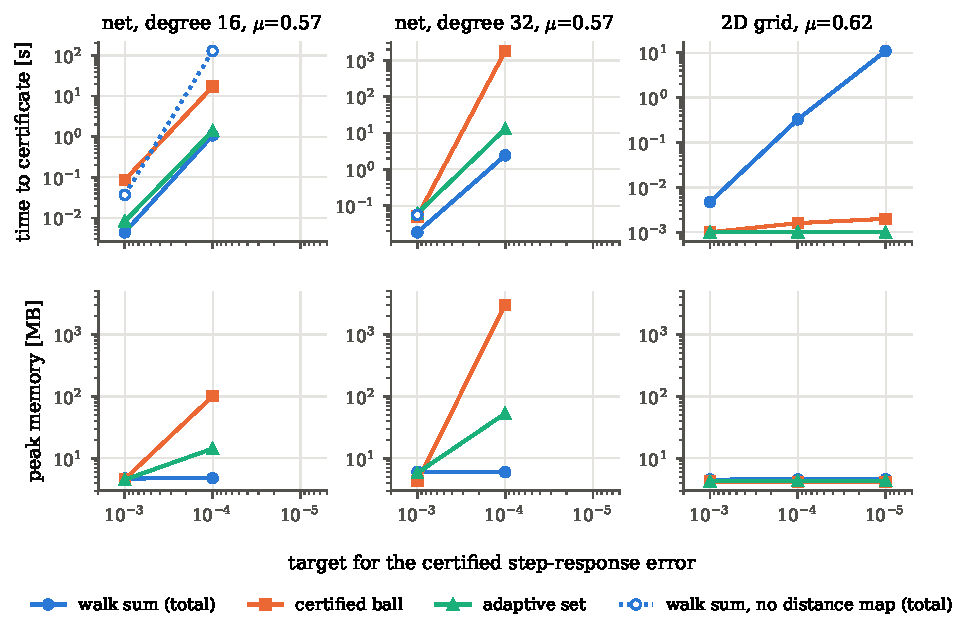
\includegraphics[width=0.85\textwidth]{figures/fig_crossover_v2.pdf}
\caption{Time to a certified step-response error from scratch (top) and peak memory of the process (bottom) for three of the graphs of Table~\ref{tab:crossover}. Walk sum: cumulative time of the threshold search, with the shared distance information (solid) and without a distance map (dotted, time only). Targets not reached by a method are omitted; on the two networks no method reached $10^{-5}$. Times below $10^{-3}$~s are plotted at $10^{-3}$~s; re-timed rows of Table~\ref{tab:crossover} enter as medians.}\label{fig:crossover}
\end{figure*}

\subsection{Separated actuator and sensor}\label{sec:noncol}
The comparisons so far use a collocated sensor, a return response. A transfer response between distinct states is smaller, and a certificate is useful only if it is small compared with the response, since the certificate is absolute (Sec.~\ref{sec:batch}). Table~\ref{tab:noncol} therefore sets the target to 10\% and 1\% of the peak of the step response. It places the sensor 2 and 4 hops from the actuator on the degree-4 network, 1 and 2 hops away on the degree-16 network, and 2 and 4 sites away on the grid. The networks use a radius-4 distance map, so that the sensor lies inside it. The peaks range from $2.8\times10^{-4}$ (two hops, degree 4) and $3.6\times10^{-4}$ (one hop, degree 16) down to $6.4\times10^{-6}$ (two hops, degree 16) and $9.7\times10^{-7}$ (four hops, degree 4).

On the degree-16 network the walk sum kept its runtime advantage. On that network with the sensor one hop away, at 1\% of the peak, the walk sum took 0.05~s, the adaptive set 0.15~s and the ball 25~s with $8.7\times10^5$ states. Two hops away, at 10\% of a peak of $6.4\times10^{-6}$, the walk sum took 0.18~s and 7.1~MB, the adaptive set 1.8~s and 16~MB with 56\,224 states, and the ball 676~s and 1.3~GB with $1.3\times10^7$ states; the 1\% target was not attempted there. On the degree-4 network the walk sum and the adaptive set both finished within 0.02~s at every separation, too fast to rank, and the adaptive set used slightly less memory; the ball needed up to 0.4~s, because a ball that must reach a distant sensor is large in every direction. On the grid the local methods again finished in under 10~ms, while the walk sum needed 0.7~s at four sites and 1\% of the peak. The distance map accounts for the higher memory of the walk sum on the degree-16 network (7.2~MB, of which about 3~MB is the radius-4 map). In every case the three outputs agreed within the sum of their certificates.

\begin{table*}[t]
\footnotesize\setlength{\tabcolsep}{2.6pt}
\caption{Separated actuator and sensor: step response at a sensor $d$ hops from the actuator, certified to 10\% and 1\% of its peak (the peak was estimated by adaptive runs with a certificate below 3\% of it). Distance information: breadth-first map of radius 4 on the networks, Manhattan distance on the grid. Walk sum: certificate, walk prefixes, cumulative time of the threshold search from scratch, peak memory. Ball (around the actuator, containing the sensor) and adaptive set: states, time from scratch and peak memory. $^\dagger$Target not reached within 1800~s. $^\S$Adaptive set stopped at its node limit without reaching the target.}\label{tab:noncol}
\begin{ruledtabular}
\begin{tabular}{lcccc|cccc|cccc|ccc}
 & & & & & \multicolumn{4}{c|}{walk sum} & \multicolumn{4}{c|}{certified ball} & \multicolumn{3}{c}{adaptive set}\\
graph & $\mu$ & $d$ & peak & target & cert. & prefixes & [s] & MB & $R$ & states & [s] & MB & states & [s] & MB\\\hline
net, $\Delta=4$ & 0.36 & 2 & $2.8\times10^{-4}$ & 10\% & $2.9\times10^{-6}$ & $3.0\times10^{2}$ & $<0.01$ & 4.4 & 4 & 161 & $<0.01$ & 4.1 & 20 & $<0.01$ & 4.1 \\
net, $\Delta=4$ & 0.36 & 2 & $2.8\times10^{-4}$ & 1\% & $1.3\times10^{-6}$ & $5.5\times10^{2}$ & $<0.01$ & 4.5 & 5 & 485 & $<0.01$ & 4.2 & 59 & $<0.01$ & 4.2 \\
net, $\Delta=4$ & 0.36 & 4 & $9.7\times10^{-7}$ & 10\% & $4.0\times10^{-8}$ & $5.7\times10^{3}$ & $<0.01$ & 4.4 & 8 & 13121 & 0.11 & 5.6 & 494 & $<0.01$ & 4.3 \\
net, $\Delta=4$ & 0.36 & 4 & $9.7\times10^{-7}$ & 1\% & $8.5\times10^{-9}$ & $2.4\times10^{4}$ & 0.01 & 4.5 & 9 & 39365 & 0.39 & 8.5 & 1452 & 0.02 & 4.4 \\
net, $\Delta=16$ & 0.40 & 1 & $3.6\times10^{-4}$ & 10\% & $1.6\times10^{-5}$ & $1.4\times10^{3}$ & $<0.01$ & 7.2 & 4 & 57857 & 1.14 & 10.6 & 257 & 0.01 & 7.0 \\
net, $\Delta=16$ & 0.40 & 1 & $3.6\times10^{-4}$ & 1\% & $3.0\times10^{-6}$ & $1.2\times10^{4}$ & 0.05 & 7.2 & 5 & $8.7\times10^{5}$ & 25 & 100.7 & 3857 & 0.15 & 7.2 \\
net, $\Delta=16$ & 0.40 & 2 & $6.4\times10^{-6}$ & 10\% & $6.1\times10^{-7}$ & $8.3\times10^{4}$ & 0.18 & 7.1 & 6 & $1.3\times10^{7}$ & 676 & 1274.4 & 56224 & 1.84 & 16.1 \\
grid & 0.45 & 2 & $5.6\times10^{-4}$ & 10\% & $2.6\times10^{-5}$ & $1.1\times10^{3}$ & $<0.01$ & 4.5 & 5 & 61 & $<0.01$ & 4.2 & 20 & $<0.01$ & 4.1 \\
grid & 0.45 & 2 & $5.6\times10^{-4}$ & 1\% & $5.3\times10^{-6}$ & $7.4\times10^{3}$ & $<0.01$ & 4.5 & 7 & 113 & $<0.01$ & 4.1 & 44 & $<0.01$ & 4.3 \\
grid & 0.45 & 4 & $4.3\times10^{-6}$ & 10\% & $3.9\times10^{-7}$ & $4.3\times10^{4}$ & 0.02 & 4.4 & 9 & 181 & $<0.01$ & 4.2 & 56 & $<0.01$ & 4.2 \\
grid & 0.45 & 4 & $4.3\times10^{-6}$ & 1\% & $3.1\times10^{-8}$ & $9.9\times10^{5}$ & 0.72 & 4.5 & 11 & 265 & $<0.01$ & 4.2 & 75 & $<0.01$ & 4.2 \\
\end{tabular}
\end{ruledtabular}
\end{table*}



\subsection{Stiffness}\label{sec:stiff}
Exact integration of the diagonal makes the cost of the walk sum depend only weakly on stiffness that resides in the diagonal. To test this we drew the thermal capacities of the $317\times317$ grid log-uniformly over $s_C$ decades below one; the comparison ratios, and with them the walk structure, do not depend on the capacities, while $\|A\|_1$ grows from 26 ($s_C=0$) to 193, 1921 and 19\,157 ($s_C=1,2,3$). Table~\ref{tab:stiff} lists the results. The walk sum visited the same 112\,429 walk prefixes at every $s_C$ and took 0.08 to 0.16~s; the increase comes from the squaring levels of the divided-difference kernel, which grew from 2 to 11. Full-system \texttt{expm\_multiply}, whose cost grows with $\|A\|t$, took 5.4, 6.4, 92 and 236~s, and the implicit BDF integrator, nearly insensitive to stiffness but slow at the tolerance needed to match ($10^{-10}$ relative), 123 to 150~s.

The local methods need only a few states here: the certified ball 113 and the adaptive set 57, at the walk sum's certificate. With the compiled explicit Taylor integrator their cost grows with $\|A\|$. The ball took 0.001, 0.006, 0.07 and 0.67~s for $s_C=0$ to 3, and the adaptive set 0.005, 0.008, 0.04 and 0.33~s, so the local methods are faster for $s_C\le2$ and the walk sum is faster at $s_C=3$. Solved with SciPy's BDF integrator, the ball took 0.3 to 0.5~s at every $s_C$, most of it interpreter overhead. A compiled implicit integrator on the ball would presumably remove the stiffness dependence of the local methods as well; we did not implement one. All methods agreed with the walk sum within its certificate.

\begin{table}[t]
\footnotesize\setlength{\tabcolsep}{1.8pt}
\caption{Stiffness sweep on the $317\times317$ thermal grid (capacities log-uniform over $s_C$ decades; step response, $t\le5$, $N=1.0\times10^5$). $\|A\|_1$ is the bound reported by the walker. Times in s; walk-sum memory is the process peak in MB. Full grid: SciPy \texttt{expm\_multiply} (Taylor) and variable-order BDF. Certified ball (113 states): compiled Taylor integrator with certified time truncation, and SciPy BDF. Adaptive set (57 states): compiled Taylor integrator. Local methods are certified at the walk sum's certificate.}\label{tab:stiff}
\begin{ruledtabular}
\begin{tabular}{rr|rrr|rr|rr|r}
 & & \multicolumn{3}{c|}{walk sum} & \multicolumn{2}{c|}{full grid} & \multicolumn{2}{c|}{ball} & adapt.\\
$s_C$ & $\|A\|_1$ & prefixes & time & mem. & Taylor & BDF & Taylor & BDF & Taylor\\\hline
0 & 26 & 112429 & 0.10 & 4.5 & 5.43 & 123 & $<0.01$ & 0.31 & $<0.01$ \\
1 & 193 & 112429 & 0.07 & 4.6 & 6.37 & 132 & $<0.01$ & 0.49 & $<0.01$ \\
2 & 1921 & 112429 & 0.08 & 5.0 & 92 & 144 & 0.07 & 0.37 & 0.04 \\
3 & 19157 & 112429 & 0.16 & 4.4 & 236 & 150 & 0.67 & 0.40 & 0.33 \\
\end{tabular}
\end{ruledtabular}
\end{table}


\subsection{Batches of times and inputs, and the number of sensors and actuators}\label{sec:batch}
On the random network with $2^{40}$ states ($\mu=0.36$, $\tau=10^{-10}$, horizon $t\le5$), increasing the number of output samples from $T=10$ to $T=1000$ changed the traversal time from 6.2 to 12.9~ms and the divided-difference workspace from 3.7 to 81~kB; the number of visited prefixes (18\,824) and of temporal row computations (1230) is independent of $T$, because the temporal work is lazy and the enumeration dominates. Adding input patterns is similarly cheap while the arithmetic stays real: one, two and four patterns (step, ramp, quadratic, decaying exponential) took 5.3, 6.3 and 7.6~ms. Including a cosine forces complex arithmetic and, with eight patterns, took 79~ms.

Reuse across input waveforms follows from Sec.~\ref{sec:piecewise}. On a network with $2^{18}$ states, one traversal produced the step kernel in 0.049~s (certificate $1.3\times10^{-7}$ per unit input), after which 100 zero-order-hold waveforms with 20 random levels each were evaluated by discrete convolution in 0.013~s in total. Propagating the full state through the same waveforms with \texttt{expm\_multiply} took 47~s per waveform (three waveforms run), and agreed with the convolution to $4.4\times10^{-9}$. The kernel route is available to any method that can produce a step response once; what the walk formulation adds is that the step, ramp and higher kernels come from the same traversal.

On the thermal grid ($\mu=0.45$, $\tau=10^{-10}$, with the Manhattan distance oracle), the traversal time grew linearly with the number of sensors (0.035, 0.049, 0.085, 0.20, 0.35~s for $p=1,2,4,8,16$ adjacent sensors, each a separate root) and sublinearly with the number of actuators (0.034 to 0.22~s for $m=1$ to 16, sharing traversals). Separating sensor and actuator by $d$ hops reduces the response by an order of magnitude or more per hop (from $7.0\times10^{-2}$ at $d=0$ to $8.9\times10^{-11}$ at $d=8$) while the certificate at fixed $\tau$ stays near $10^{-6}$, so from $d\approx4$ on the certificate exceeds the response: certificates are absolute, and a small separated response needs a proportionally smaller threshold. The distance oracle reduced the number of visited prefixes by a factor of 2.4 at $d=0$ and 29 at $d=8$.

\subsection{Unfavorable regimes}\label{sec:hard}
\begin{figure}[t]
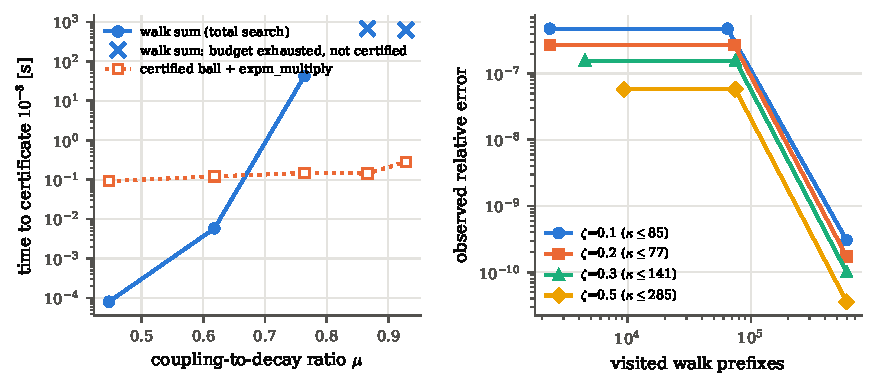
\includegraphics[width=\linewidth]{figures/fig_hard.pdf}
\caption{Unfavorable regimes. Left: time to reach a certificate of $10^{-3}$ on the step response of the $317\times317$ thermal grid as the coupling-to-decay ratio $\mu$ approaches one; for the walk sum the total time of the threshold search, with crosses where the search stopped without a certificate (plotted at the time spent; the next attempt would have exceeded the 900~s budget). Right: oscillator network in local modal coordinates; observed error relative to the response against the number of visited walk prefixes, for four damping ratios; $\kappa$ is the largest cancellation indicator over the time grid.}\label{fig:hard}
\end{figure}

\paragraph*{Coupling-to-decay ratio near one.} On the $317\times317$ thermal grid we lowered the convective loss until $\mu$ approached one and asked both methods for a certificate of $10^{-3}$ on the step response (Fig.~\ref{fig:hard}, left). The walk sum needed $8\times10^{-5}$~s at $\mu=0.45$, $6\times10^{-3}$~s at $\mu=0.62$ and 42~s at $\mu=0.76$ (total search time). At $\mu=0.87$ and $\mu=0.93$ it did not reach the target within the 900~s budget; the best certificates were $3.1\times10^{-2}$ and $0.41$, after visiting about $10^8$ and $5\times10^7$ prefixes in the last attempt. The certified ball needed radii 2 to 43 and at most 3785 states, and took 0.1 to 0.3~s in SciPy at every $\mu$. On a lattice this is the expected outcome: the ball grows polynomially with the radius while the walk count grows exponentially with the depth.

\paragraph*{Oscillatory dynamics and cancellation.} A $31\times31$ network of unit masses on grounding springs with dampers (damping ratio $\zeta$) and weak neighbor springs ($\kappa=0.05$) is a stable second-order system whose scalar diagonal splitting would place the local oscillation into the couplings. We therefore transformed each unit to its local modal coordinates, a $2\times2$ change of basis per unit, which leaves complex conjugate diagonal entries $-\zeta\omega\pm i\omega\sqrt{1-\zeta^2}$ and complex couplings ($N=1922$). The walk sum of the velocity response to a force at the same unit, computed in complex arithmetic, reproduced the real physical kernel with imaginary parts below $2\times10^{-16}$. For $\zeta=0.5$ and $0.3$ the uniform certificate applies ($\mu=0.46$, $0.70$); for $\zeta=0.2$ and $0.1$, $\mu=1.02$ and $2.0$ and only the finite-horizon certificate is available, which on $t\le5$ still certified $7\times10^{-6}$ and $1\times10^{-5}$ at $\tau=10^{-10}$ (observed errors $1.7\times10^{-10}$ and $3.0\times10^{-10}$ relative to a response of order one). The cost was the same at all four damping ratios, about $6\times10^5$ visited prefixes and 0.7~s, because over this short horizon the bounds are dominated by the couplings. The cancellation indicator, however, was 77 to 285: contributions of opposite phase cancel, and rounding errors are amplified by that factor; at the smallest threshold the observed errors were still dominated by truncation. For longer horizons the finite-horizon bound grows like $e^{\beta t}$, so for lightly damped oscillators observed over many periods we expect the cost to rise quickly; we did not test such horizons.

\paragraph*{Directed transport.} On an upwind advection chain with weak back-diffusion, $\dot x_i=-(a+\ell_i+\epsilon)x_i+a\,x_{i-1}+\epsilon\,x_{i+1}$ ($a=5$, $N=4000$), the walk sum is exact and essentially free without back-diffusion (27 prefixes visited, error $3\times10^{-16}$), because only one walk connects the actuator to a downstream sensor. Back-diffusion introduces excursions: with $\epsilon=0.2$, a sensor 20 sites downstream cost $2.4\times10^7$ visited prefixes and 34~s (certificate $6.7\times10^{-7}$, observed error $3.9\times10^{-8}$), and with $\epsilon=1$ the collocated response alone cost $6.8\times10^8$ visited prefixes and 110~s, against 0.2~s for \texttt{expm\_multiply} on the whole chain. For sensors 10 and 20 sites downstream at $\epsilon=1$ the traversal reached its 600~s limit (about $10^9$ and $2.5\times10^8$ prefixes) without a valid certificate; the partial sums were off by 11\% and 59\% of the response.

\paragraph*{Transient growth.} A regime in which only the finite-horizon bound applies is a directed chain with strong forward coupling, $\dot x_i=-(h_i+\epsilon)x_i+a\,x_{i-1}+\epsilon\,x_{i+1}$ with $a=3$, $h_i\in[0.75,1.25]$ and $N=2000$, for which $\mu$ is between 3 and 4 and $\max_{t\le5}\|e^{tA}\|_2\approx3\times10^4$ (computed on the leading 300 states). Without back-coupling ($\epsilon=0$) the chain is stable, with spectral abscissa $-0.75$, but strongly nonnormal; the walk sum is exact, with 22 prefixes visited, and the observed differences from \texttt{expm\_multiply} were at the level of rounding relative to the response ($8\times10^{-15}$ relative for a sensor ten sites downstream, where the response reaches 892). With $\epsilon=0.1$ the chain is weakly unstable (abscissa $+0.12$, from the symmetrized tridiagonal form). The collocated response was certified to $2.1\times10^{-8}$ after $8.3\times10^7$ visited prefixes in 58~s, and the response five sites downstream to $6.8\times10^{-8}$ after $2.0\times10^8$ prefixes in 302~s (observed errors $3\times10^{-11}$ and $5\times10^{-10}$); ten sites downstream the traversal reached its 600~s limit. With $\epsilon=0.3$ (abscissa $+0.70$) none of the three sensor positions was certified within 600~s, and the partial sums were off by 73 to 88\% of the response. \texttt{expm\_multiply} on the whole chain took 0.15 to 0.20~s in every case. When $\beta t$ is large and the couplings allow back-and-forth excursions, the walk sum is not a competitive method.
